\chapter{Utilities}
\label{ch:utilities}

The functionalities shared between all the components of LAR
are defined in here.

@O lib/jl/utilities.jl
@{@< Aliases @>
@< Utilities @>
@}

\subsection{Tests}
As usual every function has some unit tests.

@O test/jl/utilities.jl
@{using Base.Test
include("../../lib/jl/utilities.jl")

@< Utilities tests @>
@}


%%%%%%%%%%%%%%%
\section{Types}

To store vertices and cells boundary matrices, 
we use types already built in the standard Julia.
We use these aliases to standardize the types used 
throughout LAR. 

@D Aliases
@{const Verts = Array{Float64, 2}
const Cells = SparseMatrixCSC{Int8, Int}
const Cell = SparseVector{Int8, Int}
@}




%%%%%%%%%%%%%%%%%%%%%%%%
\section{Bounding boxes}
\label{sec:bboxes}

Bounding boxes are essential in many steps of many
algorithms in LAR. Here we present a method for building
and performing containment tests on n-dimensional bounding boxes.

@D Utilities
@{function bbox(vertices::Verts)
    minimum = mapslices(x->min(x...), vertices, 1)
    maximum = mapslices(x->max(x...), vertices, 1)
    minimum, maximum
end

function bbox_contains(container, contained)
    b1_min, b1_max = container
    b2_min, b2_max = contained
    all(map((i,j,k,l)->i<=j<=k<=l, b1_min, b2_min, b2_max, b1_max))
end
@}


%%%%%%%%%%%%%%%%%%%%%%%%%%%%%%%
\section{Face area calculation}
\label{sec:face_area}

\begin{figure}[h]
    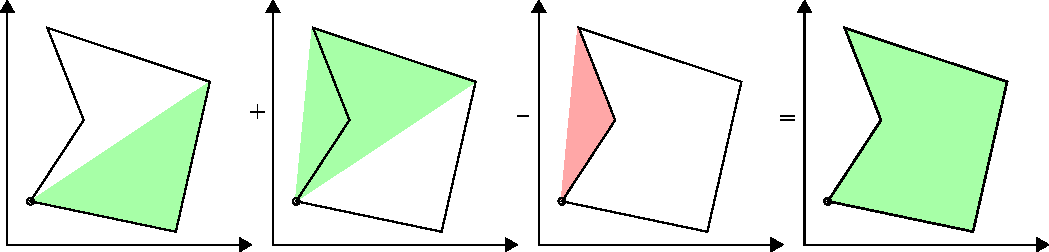
\includegraphics[width=\textwidth]{./img/ch5-1.pdf}
    \caption{Hello}
\end{figure}
\noindent
To compute the area of a generic (convex or concave) face,
we pick a pivot vertex of the face and then we iterate over
every edge of the face calculating the area of the triangle
made by the pivot vertex and the ordered extremes of the current edge.
The area of the full face is the sum of the areas of the single triangles.
This works because of the single triangles we compute the signed area with
this formula:
\begin{gather*}
    A = \frac{1}{2}
    \begin{vmatrix}
        p_{1x} & p_{1y} & 1 \\
        p_{2x} & p_{2y} & 1 \\
        p_{3x} & p_{3y} & 1
    \end{vmatrix}
\end{gather*}
Where $p_1$, $p_2$ and $p_3$ are the vertices of the triangle ($p_1$ is the pivot vertex). 
Please notice that the result of this formula will be negative only if these vertices 
are arranged in clockwise order.

@D Utilities
@{function face_area(V::Verts, EV::Cells, face::Cell)
    function triangle_area(triangle_points::Verts)
        ret = ones(3,3)
        ret[:, 1:2] = triangle_points
        return .5*det(ret)
    end

    area = 0
    ps = [0, 0, 0]

    for i in face.nzind
        edge = face[i]*EV[i, :]
        skip = false

        for e in edge.nzind
            if e != ps[1]
                if edge[e] < 0
                    if ps[1] == 0
                        ps[1] = e
                        skip = true
                    else
                        ps[2] = e
                    end
                else
                    ps[3] = e
                end
            else
                skip = true
                break
            end
        end

        if !skip
            area += triangle_area(V[ps, :])
        end
    end

    return area
end
@}

\subsection{Tests}

\begin{center}
    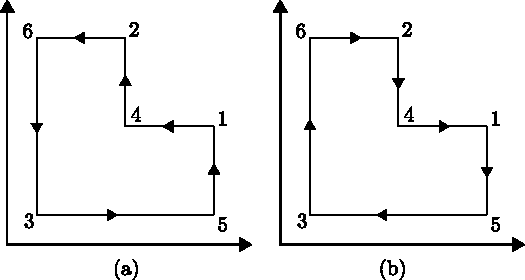
\includegraphics{./img/ch5-2.pdf}
\end{center}
\noindent Consider the two faces drawn above, they must have complimentary area.
Let's build the example in LAR.
@D Utilities tests
@{@@testset "Face area calculation test" begin
    V = Float64[2 1; 1 2; 0 0; 1 1; 2 0; 0 2]
    EV = spzeros(Int8, 6, 6)
    EV[1, [1, 4]] = [-1, 1]; EV[2, [2, 4]] = [-1, 1]
    EV[3, [2, 6]] = [-1, 1]; EV[4, [3, 6]] = [-1, 1]
    EV[5, [3, 5]] = [-1, 1]; EV[6, [1, 5]] = [-1, 1]
    FE = spzeros(Int8, 2, 6)
    FE[1, :] = [ 1 -1  1 -1  1 -1]
    FE[2, :] = [-1  1 -1  1 -1  1]

    @@test face_area(V, EV, FE[1,:]) == -face_area(V, EV, FE[2,:])
end
@}

%%%%%%%%%%%%%%%%%%%%%%%%
\section{Skeletal merge}

It is generally useful to have a utility to merge the skeletons of
two $d=2$ cellular complexes.

@D Utilities
@{function skel_merge(V1::Verts, V2::Verts, EV1::Cells, EV2::Cells)
    V = [V1; V2]
    EV = spzeros(Int8, EV1.m + EV2.m, EV1.n + EV2.n)
    EV[1:EV1.m, 1:EV1.n] = EV1
    EV[EV1.m+1:end, EV1.n+1:end] = EV2
    V, EV
end
@}